\begin{comment}
* Labeling details
- UI, filtering strategy
- Statistics
- Payment
- Timing
- Effectiveness

* General model training
- roberta finetuning
- 4 random seeds
- 3 random samples

* Task 1 - sentiment analysis, generalization accuracy
- 
- 
- 

* Task 2 - NLI, challenge set

* Task 3 - QQP checklist

\end{comment}

\newcommand{\maug}{\texttt{aug}\xspace}
\newcommand{\mcomp}{\texttt{comp}\xspace}


\section{Application 1: Data Collection}
\label{sec:app_label}




Prior work has shown that manually generated perturbations are helpful for evaluating models' decision boundaries (\eg collecting contrast sets~\cite{gardner2020contrast}), and for data augmentation~\cite{kaushik2019learning, kaushik2020explaining, teney2020learning}.
We label our perturbations in crowdsourcing tasks, and verify that the automatically generated ones can serve similar purposes at a lower labeling cost~\cite{Khashabi2020MoreBF}.
\wts{Make sure to mention that prior work said even hand generation is already cheaper than hand generating new examples.}

\subsection{Tasks \& Data}

We examine both evaluation and augmentation with three classification tasks: 
\wts{Depending on the space, probably no need to be so detailed.}

\textbf{Sentiment Analysis (\sst)} aims to determine the sentiment polarity of a given sentence (\emph{positive} or \emph{negative}). 
We select Stanford Sentiment Treebank (\dsst)~\cite{socher2013recursive} as the base dataset for augmentation.
It contains sentences extracted from full movie reviews on Rotten Tomatoes, which is relatively more aligned with the training data for the perturbation model. 
While the dataset also contains finer-grained labels on subphrases, we only use full sentences.
As a result, the full training data contains 6,920 sentences.

\textbf{Natural Language Inference (\nli)} is a 3-way classification task, with inputs consisting of two sentences, a premise and a hypothesis and the three possible labels being \emph{entailment}, \emph{contradiction}, and \emph{neutral}.
 We augment the data based on \dnli~\cite{bowman-etal-2015-large}. 
 
\textbf{Duplicate Question Detection (\qqp)} analyzes whether two questions are duplicate of each other (i.e., if you have the answer to one question, whether you can infer the answer for the other one.) 
We use \dqqp as the base dataset~\cite{wang2018glue}, a collection of question pairs from the community question-answering website Quora.



\subsection{Annotation Procedure}


\paragraph{Selecting Perturbations to Label.}


\paragraph{Filtering based on labeling results.}
For 
For augmentation, 



\begin{figure}[t]
\centering
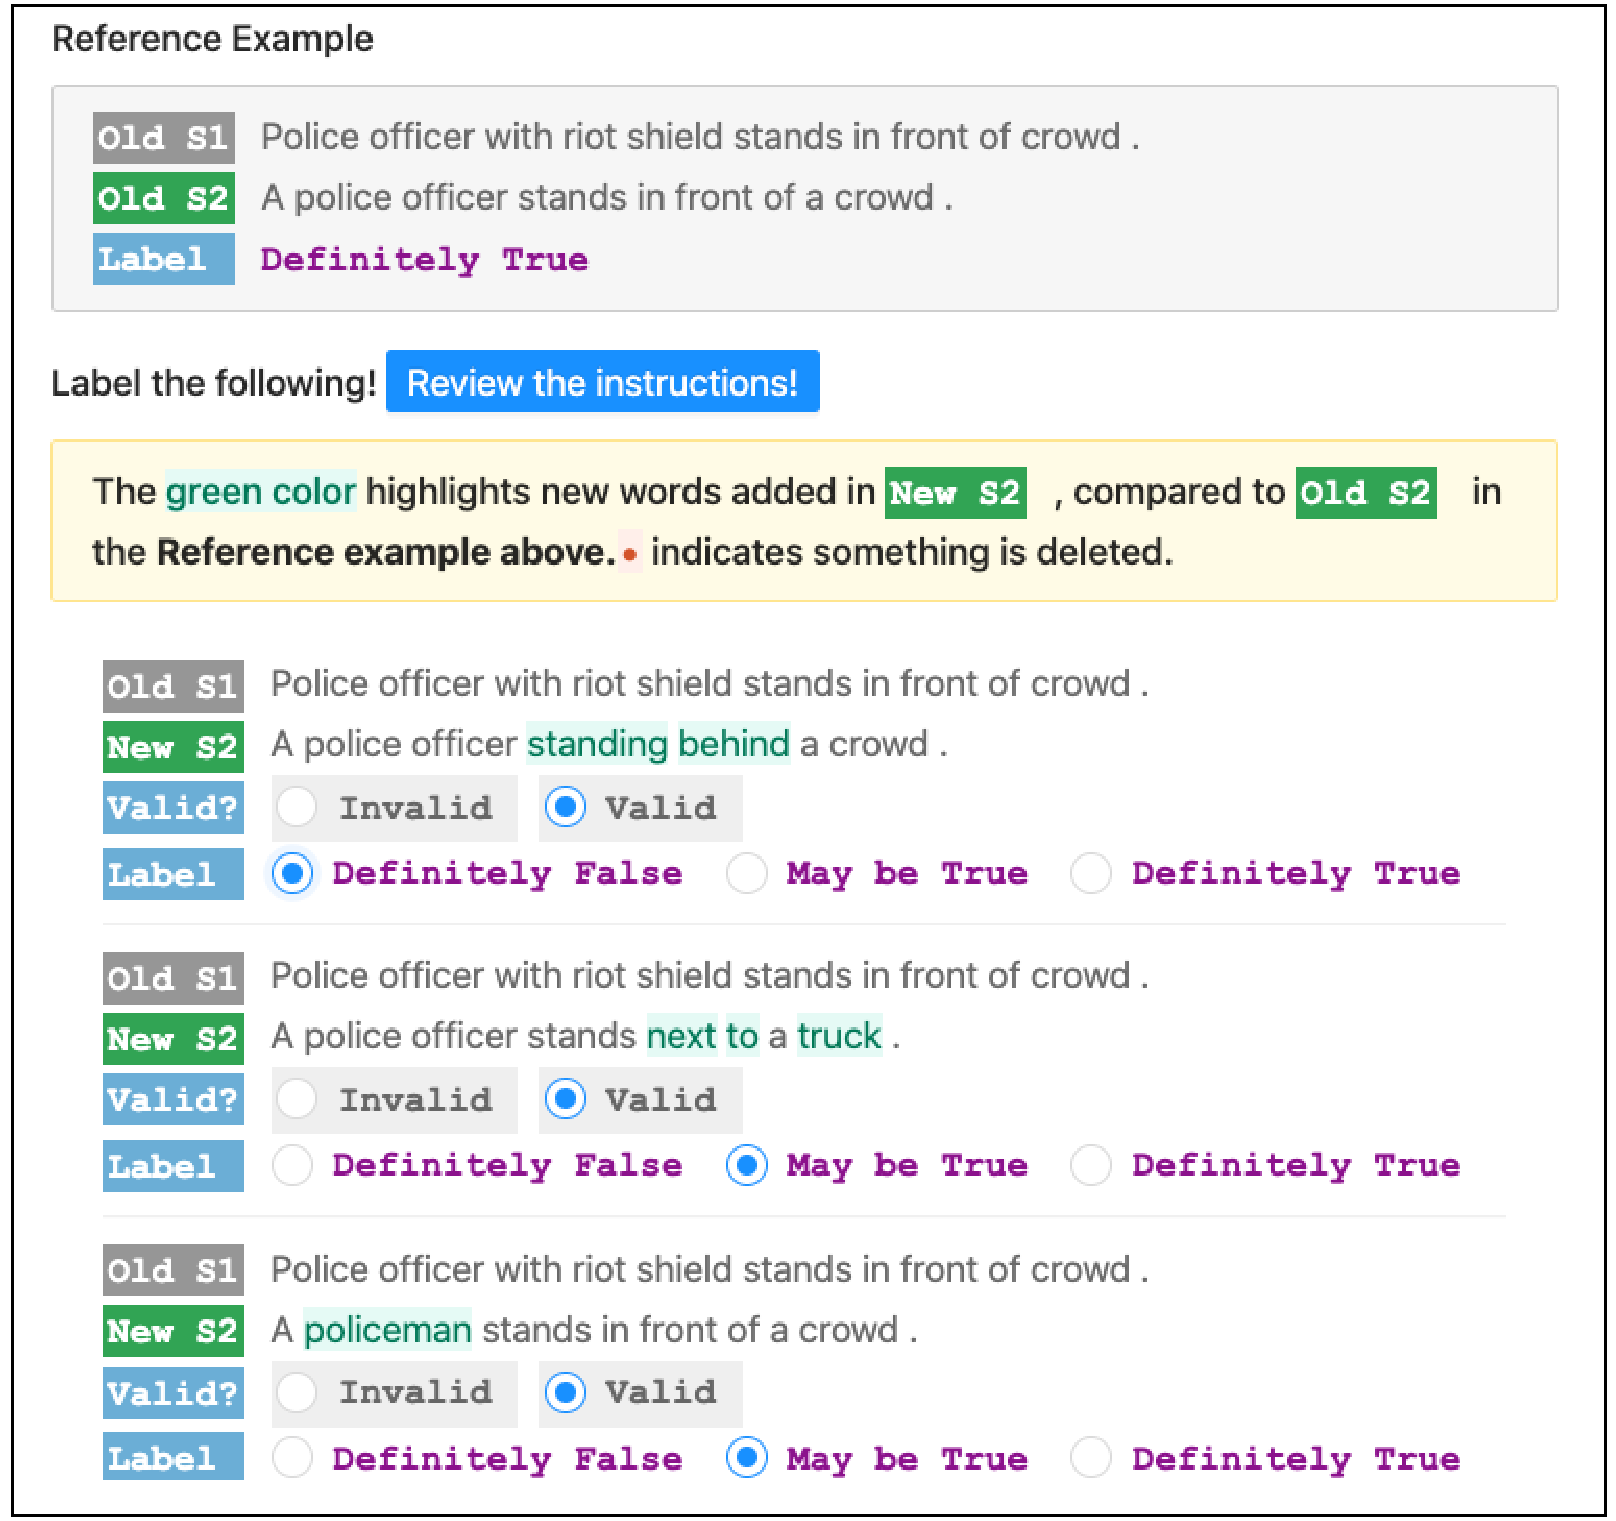
\includegraphics[width=1\columnwidth]{figures/mturk_label}
\vspace{-15pt}
\caption{A sample labeling task. For each round of labeling, the annotator is given the original instance (and its label) as a reference, and they are tasked to label three variations of the instance by (1) grammatically validity and (2) classification task label. A more detailed instruction is in \S\ref{appendix:label_instruct}. \wts{This is placeholder screenshot. Change width/height ratio, choose a better example}}
\vspace{-10pt}
\label{fig:mturk_instruction}
\end{figure}

\subsection{Contrast Set Evaluation}


\subsection{Counterfactual Data Augmentation}

%\paragraph{Datasets \& models.}
For each augmented model (\maug) in this section, we include $m$ perturbations, as well as $n$ examples sampled from the original dataset (the base examples of the perturbations will always be included).
As a baseline, we also train compensation models (\mcomp).
These models have the same $n$ original examples as their corresponding augmented models; However, the $m$ perturbations are replaced by another $m$ original samples.
Comparing with these models help highlight the effectiveness of perturbations with respect to adding the same amount of original data. 

We finetune \texttt{roberta-base} models~\cite{liu2019roberta} provided by HuggingFace Transformers~\cite{Wolf2019HuggingFacesTS}.
For each data sample, we train the models with four random seeds, and report the averaged metrics. 
For each run, we heuristically picked initial learning rates 1e-5, 2e-5, 2e-5 for \sst, \nli and \qqp, respectively, trained 20 epochs, and selected the epoch that had the highest accuracy on the corresponding validation set (1/5 of the training data size, with the same ratio of original and perturbation examples.)
\wts{Double check the reproducibility requirement to see if there's anything missing. And should I move the whole section to appendix?}
For each given $(m,n)$, we create three different samples of training data, and report the average and the variance of the samples. 
\wts{Fix the naming later: should I say perturbations, counterfactuals, or something else?}


%\textbf{Results.}
\subsubsection{Augmentation Results}
\wts{This can also be at the end.}
As detailed below, we observe that, compared to adding the same amount of original data: 
(1) The perturbation augmentation helps improve models' generalization accuracies on out-of-domain datasets, challenge sets and contrast sets, as well as CheckList testing results~\cite{checklist:acl20}.
Critically, the improvement maintains even when the augmentation size is small (\eg when $m/n<10\%$).
\wts{change number.}
(2) Meanwhile, it can maintain the in-domain accuracy.
(3) However, random samples of augmentation may be insufficient. Rather, the data should be selected based on particular data slices that needs improvements. 
Active learning might be a promising future direction.
\wts{Maybe active learning should be in future work.}
(4) The ratio of the original data and the new data is also important. Flipping out too much original data may decrease the diversity of vocabulary and syntactic structures, and therefore hurting the model performance.
\wts{See from the results if we want this takeaway.}

\paragraph{\sst.}
 Similar to \citet{kaushik2019learning}, we evaluate \sst model's generalization accuracy on out of domain datasets, including review datasets (IMDb movie review Yelp~\cite{} and Amazon~\cite{}), Twitter dataset (Senti140~\cite{} and SemEval 2017~\cite{}), and contrast sets on IMDB movie review (IMDB Contrast~\cite{} and IMDb Contrast-CAD~\cite{})  \wts{citation.}
For each dataset, we randomly selected up to 2,000 examples.
\wts{check number.}
As shown in Table~\ref{table:aug_sst}, 
\wts{Add result}

\paragraph{\nli.}
Unlike the gain in \sst, when we added random perturbations, we did not observe any improvement on any datasets.
We suspect a large number of perturbations are teaching the model patterns that it has already learned (\eg perturbations contrasting subjects ``man'' and ``woman'' may be unnecessary.) 
%For example, While flipping the from ``man'' to ``woman'' is a perfectly valid lexical change, the existing \dnli dataset already cover data points contrasting the subject of two sentences.
Instead, we prioritize perturbations that can improve error cases identified by \citet{kim2019probing} (we refer to the dataset as DNC).
We follow \citet{chen2019slice}'s data slicing strategies, and gathered data points with prepositions, comparative adjectives, negations, quantifiers, and antonyms\footnote{We extended their Appendix A.1 to include more cases of \eg comparative adjectives or negations using POS tags and parsing structures.}.
We further enforce changes on the corresponding patterns by blanking out the identified patterns, so to enforce changes on the corresponding patterns.
For example, to hopefully get an augmentation focused on prepositions like \exinline{His surfboard is \swap{beneath}{lying on} him}, we first filter examples with prepositions like ``beneath'', and generate blanked sentences like \exinline{\ctrltag{[resemantic/lexical]} His surfboard is \BLANK him.}
\footnote{All examples shown are actual generations of the model. \wts{Move this footnote to where it first occurs.}}

As a result, \maug was able to perform better on DNC (Table~\ref{table:aug_nli}), while maintaining in-domain (on SNLI test set) and out-of-domain accuracies (on MNLI matched and mismatched~\cite{}).
As shown in Figure~\ref{}, higher ratios of augmentation data is more useful. 
That said, just adding $N\%$ data is sufficient to boost the performance to some extent.
Because DNC includes pairs of probing examples (one from the original MNLI~\cite{} and one manually probed for a given linguistic pattern), we can safely conclude that the model did not overfit to a new pattern (i.e., it does not improve on \exinline{lying on} by sacrificing performances on \exinline{beneath.})
The model also performs better on some other challenge sets that are not our initial improvement targets.


\paragraph{\qqp.}
Similar to \nli, we focus on data slices whose perturbations may be more helpful on failed tests identified in CheckList, \eg the entity orders (slicing on examples with multiple entities, and \ctrltag{shuffle} them), temporal information (\eg find examples with \exinline{before} and \BLANK it to hopefully get \exinline{after}).
Augmenting $n=$ original examples with $m=$ perturbations, we were able to reduce model failure rates on X tests (out of the X failed ones). 
In most cases, the gain on one test does not hurt its counterparts (\eg we get gains on all tests related to entity ordering.)
However, we did see one potential overfitting: While the model gets significantly better on  \texttt{more X != less X}, it sacrifices the performance on \texttt{more X == less antonym(X)}.
Future work should further strategize the sampling, such that the augmentation distributes more equally across various related or contrasting sub-cases. 

\begin{comment}
	I get more win in this case (even at the orig_size=20k)
some of the wins are on duplicate
In many cases we are not hurting too much on the counter-case (\eg the order ones ^ how can I become a person...); the only please we are definitely hurting too much is more X == less antonym(X)
I also tried doing (q1, q1'), and I think if I do this, I can also get "Irrelevant preamble with different examples.", but probably won't do much better on others, so not so sure if it's worth the effort to explain lol
\end{comment}



\begin{comment}
For testing on other datasets, we use a random subset (2000 examples) of the test sets of Amazon Reviews [45], Semeval 2017 (Twitter data) [55], and Yelp reviews [77] similarly to [34].
from Learning What Makes a Difference from Counterfactual Examples and Gradient Supervision
	
\end{comment}
